\begin{frame}
    \frametitle{Konzept}
    \framesubtitle{Ballbeschleunigung}
    \begin{columns}
        \begin{column}{0.4\textwidth}
            \begin{block}{Ballbeschleunigung}
                \begin{itemize}
                    \item Ein Rad oberhalb
                    \item<2-> BLDC Motor
                \end{itemize}
            \end{block}
            \centering
            \pause
            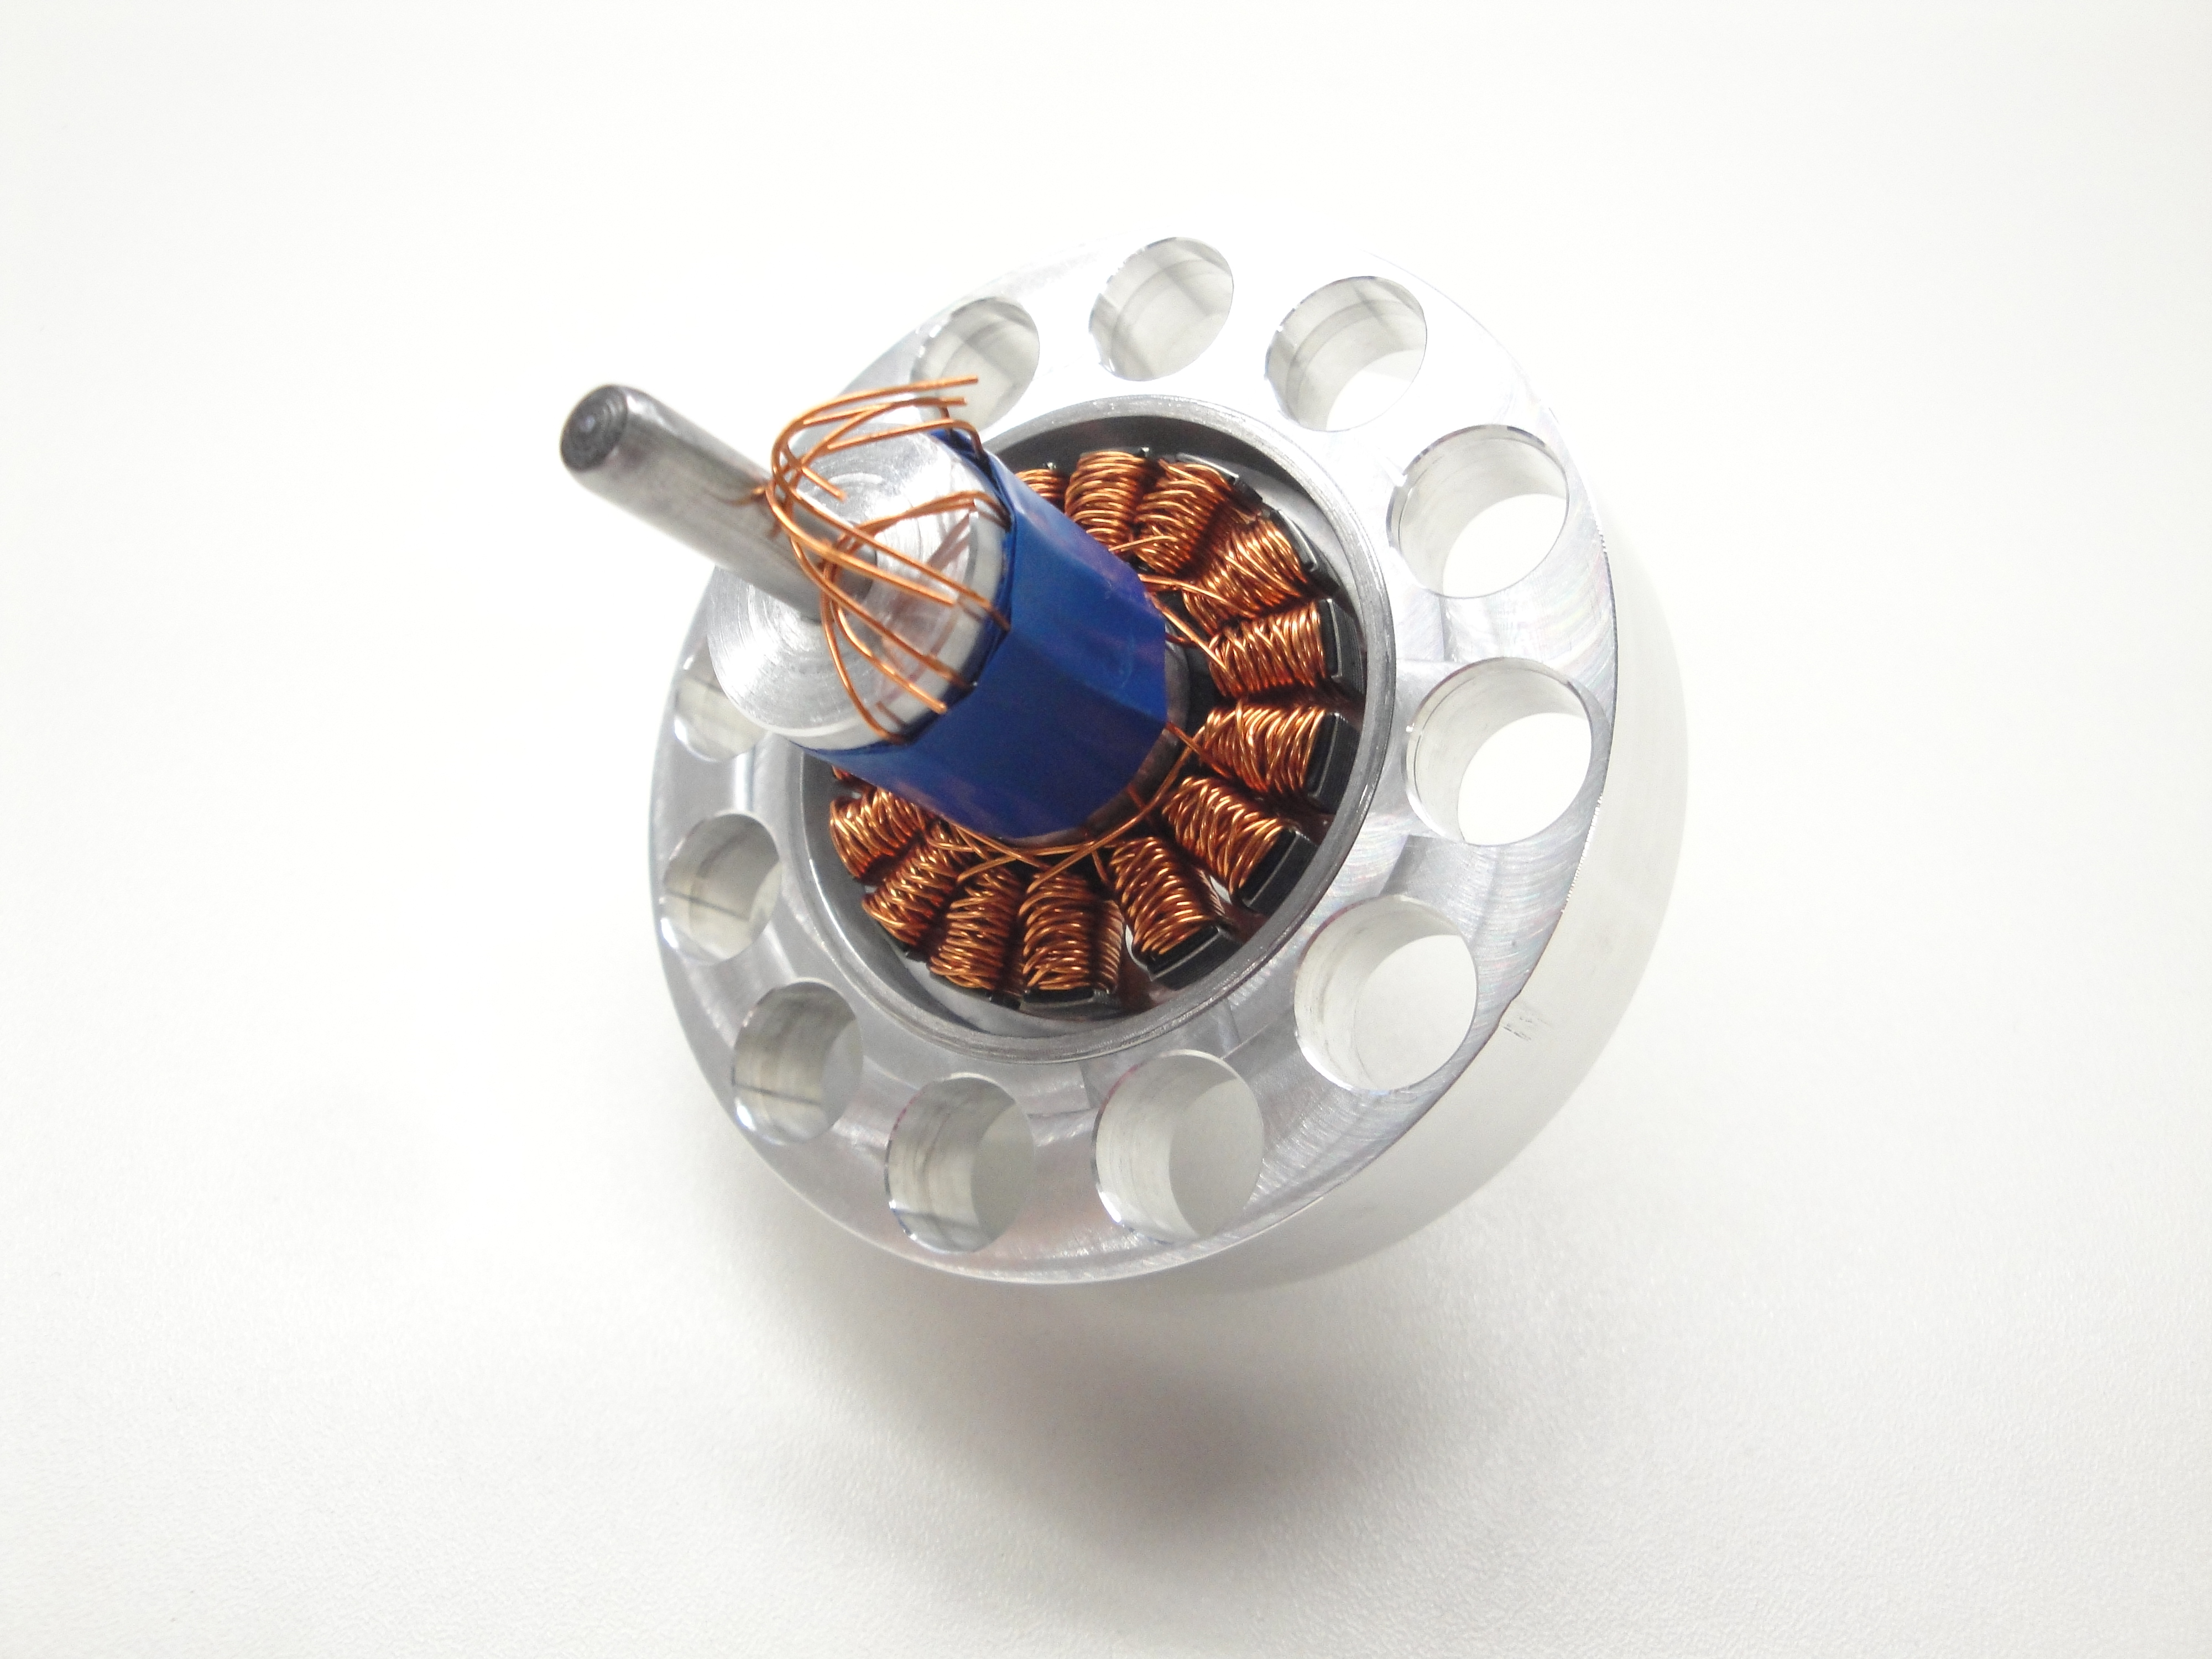
\includegraphics[width=0.8\textwidth, trim = 330mm 200mm 300mm 100mm, clip]{../fig/bldc/DSC02754.JPG}
        \end{column}
        \begin{column}{0.6\textwidth}
            \centering
            \onslide
            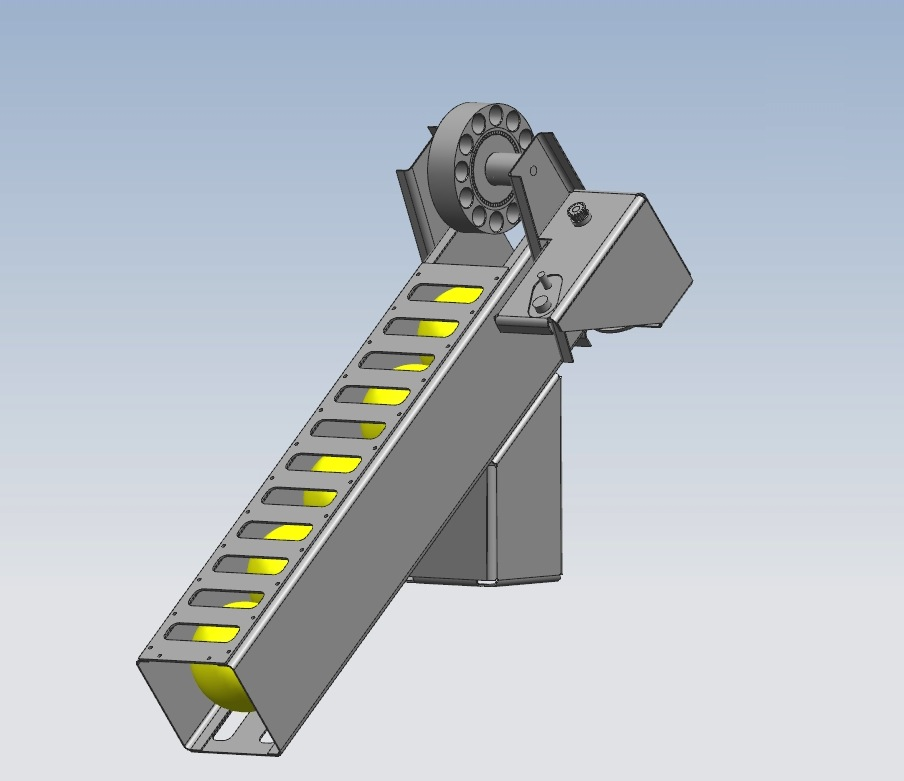
\includegraphics[width=0.8\textwidth, trim = 40mm 0mm 60mm 30mm, clip]{../doc/fig/Balllager.jpg}
        \end{column}
    \end{columns}
\end{frame}

